%======================================================================
\chapter{Implementation}
\label{ch: Chapter5}
%======================================================================

For the Implementation of this project we had to start mostly from scratch since this was a new project for Bradley and not inherited.  The main starting point is that there have bean senior project in the past that used XBees to get signal strength as well but past that there is very little overlap between them. So for this project we had to first build a robot and a remote to use for testing. Then we had to build code base to control the mobile robot that we then implement our test algorithms with.

%----------------------------------------------------------------------
\section{Robot Assembly}
\label{sec:Robot Assembly}
%----------------------------------------------------------------------

For this project we needed a Remote Target and Smart Robotic Cart that we designed and implemented from off the shelf components.  As mentioned above in \autoref{sec:System Components} some of our components came from what the school already owned as well as some we had to buy specifically for this project listed in \autoref{tab:Partslablist} and \autoref{tab:Partslablist}.

\vspace*{12pt}
\noindent
Since the school already owned the Budget Bot chassis, we opted to use these base cart chassis frames to build our Smart Robotic Cart upon.  The base Budget Bot chassis did need to be modified slightly to work with our project.  The main change was that we swapped out the motors that came with the Budget Bot for Pololu 27D Meatal Gear motors since the original motors spin at max speed is 212 RPM or 1.09m/s and the new motors max speed is 530 RPM or 2.72m/s when using the base wheels that have a diameter of 98mm.  By switching out the motors we are able to achieve our goal of  matching an average person's walking speed of 1.5m/s since the build in motors can not achieve this. The other modifications to the chassis are that a hard power switch was added to directly cut off power to the XBee modules in the reflector as well as a power indicator LED.

\begin{figure}
	\centering
	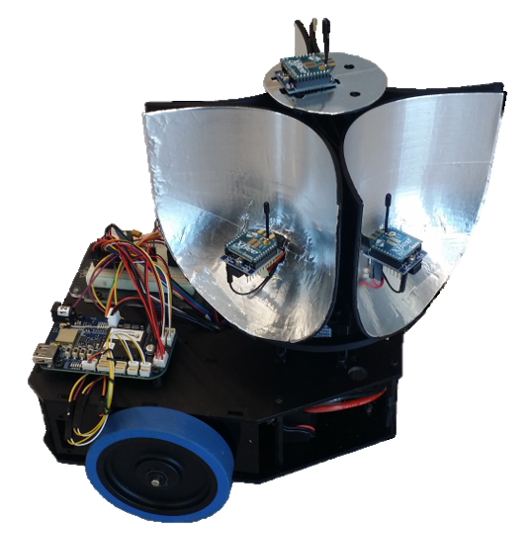
\includegraphics[width=0.5\textwidth]{figs/img/Finalized_robot.png}
	\caption{Final Version of the Robotic Cart}
 	\label{fig:FinalizedRobot}
\end{figure}

\vspace*{12pt}
\noindent
As can be seen in \autoref{fig:FinalizedRobot} our next step was to attach the Beagle Bone Blue microcomputer, XBee reflector array assembly, and breadboard to the top of the robot.  We also installed a 2-cell LiPo battery inside the body of the mobile cart that delivers power to the Beagle Bone Blue directly and power to the breadboard through the switch. \par
The power supplied to the breadboard is sent through a regulator circuit to drop it down from 7.4v from the LiPo to 3.3v.  This same circuit also is used on the remote which consists only of a 9v battery and the XBee module with this voltage regulator in between.  This voltage regulator is build out of a LM117 regulator and a 10uF ceramic capacitor between the input and output pins of the regulator as shown in \autoref{fig:PowerConverter}.

\begin{figure}
	\centering
	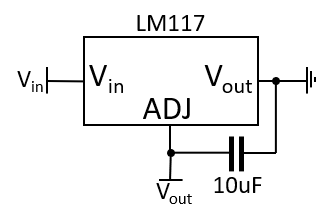
\includegraphics[width=0.5\textwidth]{figs/img/PowerConverter.png}
	\caption{Final Version of the Robotic Cart}
 	\label{fig:PowerConverter}
\end{figure}

\vspace*{12pt}
\noindent
The Reflector array assembly from \autoref{ch: Chapter3} was mounted on a stepper motor that was then attached to the robot chasse using a 3D printed bracket.  This bracket was the attached to the chasse using bolts.  Another feature of this bracket is that it had a stop block built into the top of it that is used to automatically zero the reflector array when the robot starts up.

\vspace*{12pt}
\noindent
The Xbee modules from the reflector posed a bit of a problem when it came to connecting them to the Beagle Bone Blue.  This problem comes from that the Beagle Bone Blue has five UART ports if we are using the one found in the USB and the UART-GPS along with the three normal UART ports.  This unfortunately dose not work though since UART port zero is tied to the council used to communicate with it from a computer.  Since this port is reserved for this function that reduces the number of usable ports down to four which does not work since we have five XBees in it.  Our solution to this was to use two of the GPIO pins, two of the UART ports, and a two-way multiplexer.  With this setup we can directly connect one of the UARTs to the top XBee and then rout the other four side XBee modules through the MUX so only one UART port is needed for them.


%----------------------------------------------------------------------
\section{Code Base}
\label{sec:Code Base}
%----------------------------------------------------------------------

For the project we needed some base functionality to use with the main follower program so it can interact with the other components in the system.  The Beagle Bone Blue already has a set of ports on it that we can access and control using the Robot Control Library from Strawson Design for the beagle bone blue ~\cite{Robot_Control_Library}.

\vspace*{12pt}
\noindent
For the project we also build some custom libraries on top of the Robot Control Library to hand XBee Frames, AT Commands, and the stepper motor.  The XBee frames library takes a given block of data containing our message and then packages it into a XBee Frame to send over UART to the XBee module we want to interact with.  The XBee communications library also handles received messages from the XBee module and validates the received frames integrity and extracts the message data from it.  On top of the XBee communications library we also have a library that generates AT Commands to package in the XBee Frames.  The AT Command library also handles extracting response data from the AT Response Command structure and validating it.

\begin{figure} [b]
  \centering
  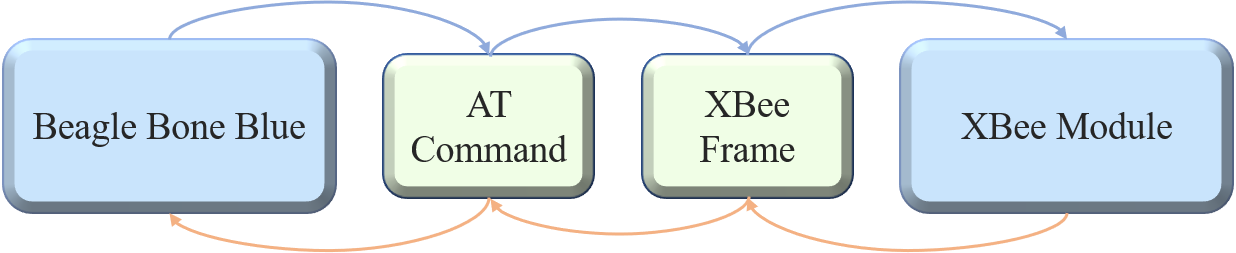
\includegraphics[width=\textwidth]{figs/img/Command Process Diagram.png}
  \caption{Process for XBee Communication over UART}
  \label{fig:CommandProcessDiagram}
\end{figure}

\vspace*{12pt}
\noindent
The final custom library is the stepper motor control library.  This library had to be written ourselves since instead of using a dedicated stepper motor controller for our project we were using two of the regular DC motor control ports that are build into the Beagle Bone Blue.  This library handled translating how many steps to turn into proper cycling of the DC motor ports to get the stepper motor to move the desired distance.  The library also helped to keep track of basic information related to the stepper motor such as what its current angel should be.

%----------------------------------------------------------------------
\section{Experimental Results}
\label{sec:Experimental Results}
%----------------------------------------------------------------------

In this project after we had the Robotic Cart, Remote Target, and a code base to handle the specifics we started testing different variants of our algorithm explained in \autoref{ch: Chapter4}. There were two main types of variants we put together, one type the stepper motor is locked preventing the reflector from turning and in the other we use the stepper motor to sweep through a set of angles.

\subsection{Rotating Reflector Tests}

The first type of test we ran was where the robot would zero out the arrays rotation with the stepper motor then move in nine degree increments taking measurements as it went. A sweep ends when the motor has turned 81 degrees since at that point with the fore sides of the reflector a full 360 degrees has bean scanned.

\vspace*{12pt}
\noindent
This method offers us a sufficiently dense set of data to base our angle predictions off of but at the cost of having to wait until a entire sweep is completed. With this data we first put together a simple test that would continuously be sweeping and moving at the same time. Though this version did successful follow the remote it was incredibly unstable.  The result of this instability was that the robot would most of the time correctly turn towards the remote and then start moving towards it but as it went it would slowly pick up a osculation in its movement until the wobble got to great and it would drive off in a random direction then find its way back into alignment and resume moving towards the remote.

\vspace*{12pt}
\noindent
The next version that used a rotating reflector as well as the final version works mostly the same as the first version but with some improvements to its navigation.  The first big fix is that we determined that the result of the osculation we were seeing in the first test was a result of turning while also rotating the reflector which would add additional rotation to the measurements in global scope.  Do to how are robot is designed we can only rotate the reflector array 90 degrees but to properly fix this rotation issue we would need to rotate the reflector more or less during a sweep to compensate for the robots rotation. Our compromise was simply to allow the robot to always move forward but to alternate between rotating the reflector and getting a measurement and then rotating the robot based on that measurement.  In this version we also added some additional windowed filters to average out the angle measurements which did help to reduce the effects of random angles from noise in the system.  We also applied offsets to each of the directional receivers revived signal strengths based of of data that we had collected while testing it when we noticed that each side had a different minimum that it would cap out at.

\subsection{Locked Reflector Tests}

The locked reflector test were some tests that we ran in between our first sweeping algorithm and our final algorithm which ultimately used sweeping. These algorithms were an attempt to reduce the time needed to get a set of measurements from the reflector by zeroing its rotation and then keeping it locked in the zeroed position.  Since the data from this is relatively sparse we tried three different ways to fill in the gaps in the data from only the four cardinal directions. The first of these three methods was to try and select a strongest direction that the signal was coming from and then witch of its two neighbor directions had the next strongest signal. With these two strengths the algorithm would then try to interpolate between these two angles based on difference of the strength between them. This method probably can work but in our implementation we ran out of time to try and tune it since it would take a fairly large amount of data to be collected to try and tune it in.

\vspace*{12pt}
\noindent
The other two methods that we tried with the locked reflector were both different variants on machine learning based on a small poll of data we had collected. The first algorithm tested was K Nearest Neighbors then followed up by a Neural Network for our final fixed rotation test.  Both of these algorithms failed to produce any meaningful results.  This would appear to be due to the fact that we had a very small pool of data to work off compared to usual attempts to use machine learning. They also with the small data pool size did not cope particularly well with the noise in the signal.

\subsection{System noise}

In both our fixed and seeping experiments a underlying issue is the amount of noise our system produces.  The first type of noise that occurs is noise from the Multipath Effect where the signals bounce off of obsticals around it adding constructing and destructive interference randomly based off of the robots surroundings.  The second noise was from internal noise in the XBees which was worse that we had expected.  We to some degree managed to isolate the XBee internal noise by using an anecoic chamber where we did see all the signals strengths become stronger but the base noise from the XBees persisted. The noise coming from the XBees tends to be about 2 to 6 dBm around the average and the change from facing towards to away from the remote is about 13 to 15 dBm.  This ranges result in the occasional measurement that flip flops which reflector is actually facing the remote. The noise can be seen in our test measurements we collected where we at set rotations record a burst of 300 measurements as seen in \autoref{fig:SensorDataGraphs}

\begin{figure}
    \centering
    \begin{subfigure}{0.50\textwidth}
        \centering
        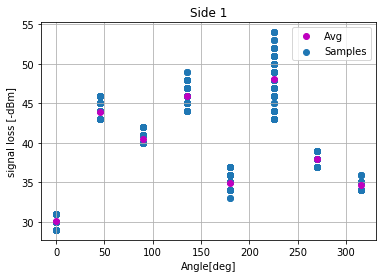
\includegraphics[width=0.95\textwidth]{figs/img/Side1_Data.png}
        \label{fig:Side1Dat}
    \end{subfigure}%
    \begin{subfigure}{0.50\textwidth}
        \centering
        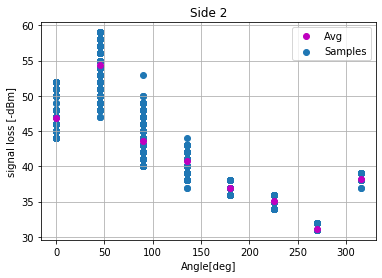
\includegraphics[width=0.95\textwidth]{figs/img/Side2_Data.png}
        \label{fig:Side2Dat}
    \end{subfigure}
        \begin{subfigure}{0.50\textwidth}
        \centering
        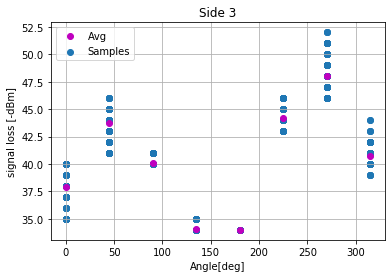
\includegraphics[width=0.95\textwidth]{figs/img/Side3_Data.png}
        \label{fig:Side3Dat}
    \end{subfigure}%
    \begin{subfigure}{0.50\textwidth}
        \centering
        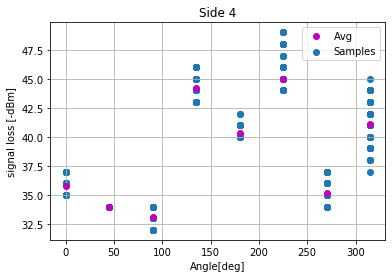
\includegraphics[width=0.95\textwidth]{figs/img/Side4_Data.png}
        \label{fig:Side4Dat}
    \end{subfigure}
    \caption{Navigation Algorithm Details}
    \label{fig:SensorDataGraphs}
\end{figure}

\subsection{Distance}

\todo[inline]{Was going back over this and realized I should add this section in will do later don't have time at this exact moment. -Darrah}

[Uhhh what?]
\todo[inline]{What am I looking at on page 23 exactly? -Darrah}
\todo[inline]{See page 23 of~\url{http://ee.bradley.edu/projects/proj2017/ekf_slam/Downloads/seniorProject_finalReport.pdf} -Dr. Miah}


\section{Simulation using Robot Simulator}

Before constructing the physical robot prototype, a simulation was performed using a commercial robot simulator CoppeliaSim. However, since RF signal behavior depends highly on the environment, the system could not be fully simulated. This section explains the steps taken to simulate the proposed robotic cart.

\vspace*{12pt}
\noindent
First, a model of the Budget Bot chassis was created in CoppeliaSim. The model is shown in Fig. \ref{fig:budgetBotModel}. The model was designed with the same dimensions as the physical chassis to accurately simulate the robot kinematics. Details on modeling a robot chassis in CoppeliaSim can be found in \autoref{ch:coppSimModeling}. Although \autoref{ch:coppSimModeling} explains the modeling of a robot chassis that is different than the Budget Bot chassis, the concepts are the same for modeling any robot chassis.
\begin{figure}
    \centering
    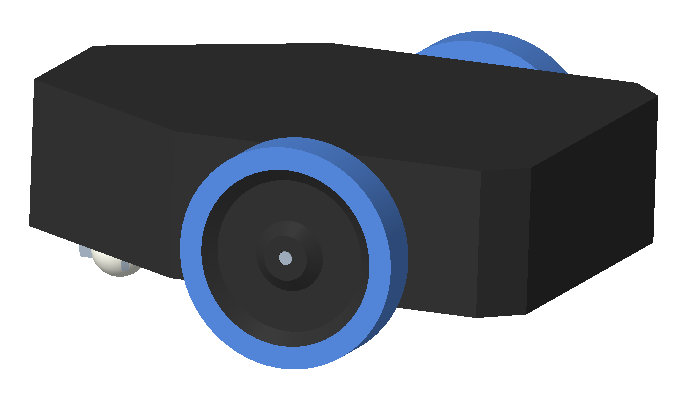
\includegraphics[width=0.6\textwidth]{figs/img/budgetBotModel.png}
    \caption{Model of Budget Bot Chassis}
    \label{fig:budgetBotModel}
\end{figure}

\vspace*{12pt}
\noindent
MATLAB code was written to control the simulation. The actual distance between the robot and the remote was measured, then random noise was added with a mean of 0 and a standard deviation of 0.07. This noisy measurement was then used in the navigation algorithm to determine how to drive the robot (see \autoref{sec:navAlgo}). An image of the simulation is shown in Fig. \ref{fig:coppSimExample}, where the blue sphere represents the remote, and the green dot represents the target point.
\begin{figure}
    \centering
    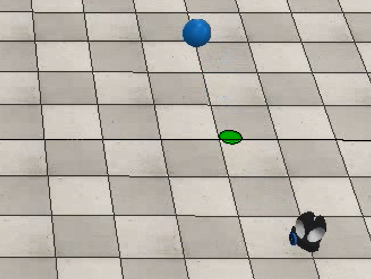
\includegraphics[width=0.5\textwidth]{figs/img/coppSimExample.png}
    \caption{CoppeliaSim Simulation}
    \label{fig:coppSimExample}
\end{figure}


%%% Local Variables:
%%% mode: latex
%%% TeX-master: "../finalReport"
%%% End:
